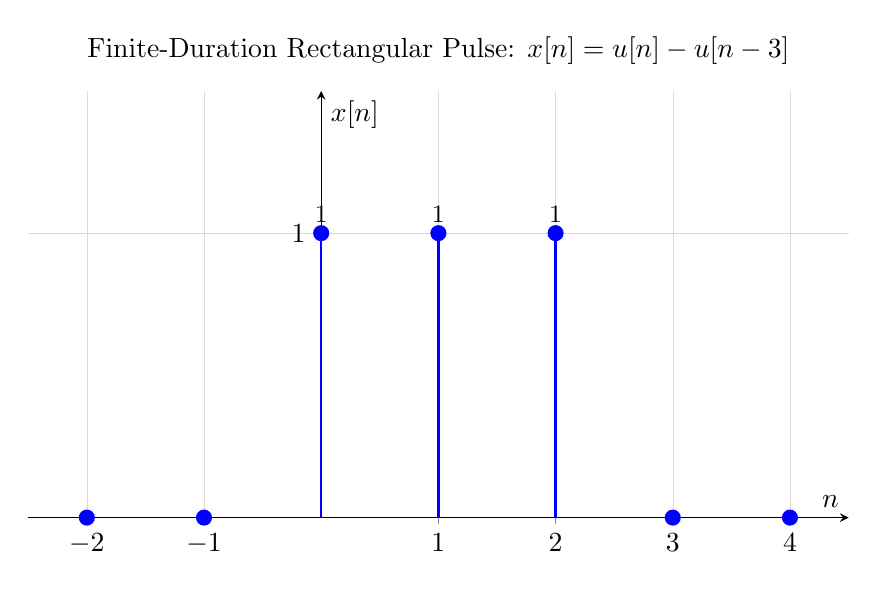
\begin{tikzpicture}
	% Define a style for our stem plots to avoid repetition
	\pgfplotsset{
		impulse/.style={
			ycomb,          % Use the 'ycomb' style for stems
			thick,          % Thickness of the stems
			mark=*,         % Marker style at the tip of the stem
			mark size=2.5pt,% Size of the marker
			blue,           % Ensure the line color is blue
			mark options={fill=blue, draw=blue}, % Explicitly set marker colors
		}
	}
	
	\begin{axis}[
		% Set the overall style
		width=12cm,
		height=7cm,
		% Title with the signal's formal definition
		title={Finite-Duration Rectangular Pulse: $x[n] = u[n] - u[n-3]$},
		% Axis labels
		xlabel={$n$},
		ylabel={$x[n]$},
		% Position axes at the origin
		axis lines=middle,
		% Set axis limits
		xmin=-2.5, xmax=4.5,
		ymin=0, ymax=1.5,
		% Set ticks at key points
		xtick={-2, -1, 0, 1, 2, 3, 4},
		ytick={1},
		yticklabels={$1$}, % Use symbolic label 'A'
		% Add a grid
		grid=major,
		grid style={line width=.1pt, draw=gray!30},
		]
		
		% Plot the non-zero impulses and add symbolic labels above them
		\addplot[
		impulse,
		nodes near coords={1}, % Display the symbol 'A' at each point
		every node near coord/.style={anchor=south, font=\small, text=black}, % Position labels
		] coordinates {
			(0, 1)
			(1, 1)
			(2, 1)
		};
		
		% Plot some zero-value points to show the signal's extent
		\addplot[impulse] coordinates {
			(-2, 0)
			(-1, 0)
			(3, 0)
			(4, 0)
		};
		
	\end{axis}
\end{tikzpicture}